% !TeX program = lualatex


\documentclass[aspectratio=169,xcolor={dvipsnames}
%,notes=only
%,notes
%,show notes on second screen=right
,handout
]{beamer}
\usetheme[background=light, numbering=fraction]{metropolis}
\usepackage{appendixnumberbeamer}
\usepackage{pgfpages}

%\usepackage[T1]{fontenc}

\usepackage{bm}

\usepackage[labelfont=bf,textfont={it}]{caption}
\usepackage{subcaption}
\captionsetup[figure]{justification=centering}
\captionsetup[subfigure]{justification=centering}

\usepackage{tikz}
\usetikzlibrary{arrows.meta, calc, fit, positioning}

%\usepackage{fontspec}
%\setsansfont{Fira Sans Mono}

\usepackage{etoolbox}
\usepackage[binary-units]{siunitx}
\robustify\bfseries
\sisetup{detect-all, range-phrase=--, range-units=single}

\usepackage[UKenglish]{babel}
\usepackage{csquotes}

\usepackage{amssymb}

\usepackage{lipsum}
\usepackage[basic]{complexity}
\usepackage[super,negative]{nth}

\usepackage{booktabs}

%bib
\usepackage[maxnames=3,maxbibnames=99,mincrossrefs=5,sortcites
,backend=bibtex
,style=authortitle
]{biblatex}
%\addbibresource{papers.bib}
%\addbibresource{confs-journs.bib}

\newcommand{\acval}[3]{\ensuremath{\operatorname{\hat{q}}(#1, #2, #3)}}
\newcommand{\wvec}[1]{\ensuremath{\bm{w}_{#1}}}

\makeatletter
\DeclareRobustCommand{\rvdots}{%
	\vbox{
		\baselineskip4\p@\lineskiplimit\z@
		\kern-\p@
		\hbox{.}\hbox{.}\hbox{.}
}}
\makeatother

% official colours
\definecolor{uofguniversityblue}{rgb}{0, 0.219608, 0.396078}

\definecolor{uofgheather}{rgb}{0.356863, 0.32549, 0.490196}
\definecolor{uofgaquamarine}{rgb}{0.603922, 0.72549, 0.678431}
\definecolor{uofgslate}{rgb}{0.309804, 0.34902, 0.380392}
\definecolor{uofgrose}{rgb}{0.823529, 0.470588, 0.709804}
\definecolor{uofgmocha}{rgb}{0.709804, 0.564706, 0.47451}

\definecolor{uofglawn}{rgb}{0.517647, 0.741176, 0}
\definecolor{uofgcobalt}{rgb}{0, 0.615686, 0.92549}
\definecolor{uofgturquoise}{rgb}{0, 0.709804, 0.819608}
\definecolor{uofgsunshine}{rgb}{1.0, 0.862745, 0.211765}
\definecolor{uofgpumpkin}{rgb}{1.0, 0.72549, 0.282353}
\definecolor{uofgthistle}{rgb}{0.584314, 0.070588, 0.447059}
\definecolor{uofgpillarbox}{rgb}{0.701961, 0.047059, 0}
\definecolor{uofglavendar}{rgb}{0.356863, 0.301961, 0.580392}

\definecolor{uofgsandstone}{rgb}{0.321569, 0.278431, 0.231373}
\definecolor{uofgforest}{rgb}{0, 0.317647, 0.2}
\definecolor{uofgburgundy}{rgb}{0.490196, 0.133333, 0.223529}
\definecolor{uofgrust}{rgb}{0.603922, 0.227451, 0.023529}

\definecolor{inferno0}{rgb}{0.001462 0.000466 0.013866}
\definecolor{inferno64}{rgb}{0.341500 0.062325 0.429425}
\definecolor{inferno128}{rgb}{0.735683 0.215906 0.330245}
\definecolor{inferno192}{rgb}{0.978422 0.557937 0.034931}
\definecolor{inferno255}{rgb}{0.988362 0.998364 0.644924}

%picky abt et al.
\usepackage{xpatch}

\makeatletter\let\expandableinput\@@input\makeatother

\xpatchbibmacro{name:andothers}{%
	\bibstring{andothers}%
}{%
	\bibstring[\emph]{andothers}%
}{}{}

%opening!

\usepackage{cleveref}
\newcommand{\crefrangeconjunction}{--}

\usepackage{fontawesome}

\addtobeamertemplate{footnote}{\vspace{-6pt}\advance\hsize-0.5cm}{\vspace{6pt}}
\makeatletter
% Alternative A: footnote rule
\renewcommand*{\footnoterule}{\kern -3pt \hrule \@width 2in \kern 8.6pt}
% Alternative B: no footnote rule
% \renewcommand*{\footnoterule}{\kern 6pt}
\makeatother

\usepackage[export]{adjustbox}
\usetikzlibrary{arrows.meta, calc, fit, positioning, shapes.misc}

%-------------------------------------%
%-------------------------------------%

\title{Reinforcement Learning in Future Networks}
\author{\vspace{-1em}\textbf{Kyle A. Simpson}\\
	\faEnvelopeO{} \href{mailto:k.simpson.1@research.gla.ac.uk}{\nolinkurl{k.simpson.1@research.gla.ac.uk}}\\
	\vspace{1em}\small{\faGithub{} \href{https://github.com/felixmcfelix}{FelixMcFelix} \hspace{0.5em} \faGlobe{} \url{https://mcfelix.me}}}
\institute{University of Glasgow}
\date{\nth{27} March, 2020}

\begin{document}
\begin{frame}
\maketitle
\end{frame}

\begin{frame}{Data-driven networking: RL in networks}
	\alert{Data-driven networking}: Automate control, optimisation, configuration of the network.
	\begin{itemize}
		\item Flow performance optimisation.
		\item Resource allocation.
		\item Adaptive response to load, intrusions, etc.
		\item Feedback loop-like.
	\end{itemize}
\end{frame}

\begin{frame}{Data-driven networking: DDoS Prevention}
	\begin{columns}
		\begin{column}{0.6\linewidth}
			\begin{figure}
				\centering
				\resizebox{\linewidth}{!}{
					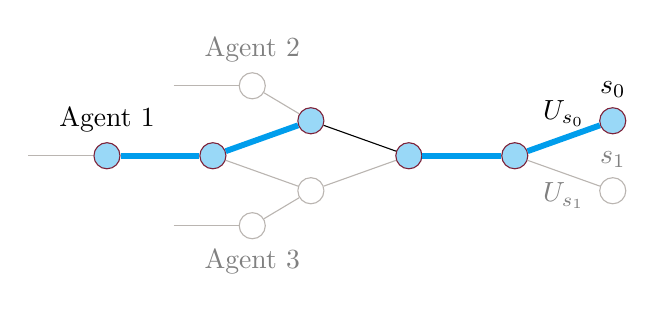
\begin{tikzpicture}[
					texts/.style = {text=black},
					labeltexts/.style = {text=gray},
					treeline/.style = {draw=uofgburgundy},
					treenode/.style = {texts, circle, centered, fill=white, treeline},
					load/.style = {fill=uofgcobalt},
					loadline/.style = {draw=uofgcobalt, line width=0.75mm},
					loadhide/.style = {fill=uofgcobalt!40!white},
					external/.style = {fill=uofgrust},
					externalhide/.style = {fill=uofgrust!40!white},
					hideline/.style = {draw=uofgsandstone!40!white},
					hidenode/.style = {treenode, hideline},
					grow'=right
					]
					\node [treenode, loadhide, label={[texts]above:Agent 1}] (mainagent) {};
					\node [treenode, loadhide, right = of mainagent] (inner0) {};
					\node [treenode, loadhide, above right = 0.2cm and 1cm of inner0] (inner1) {};
					\node [hidenode, below right = 0.2cm and 1cm of inner0] (inner2) {};
					\node [treenode, loadhide, below right = 0.2cm and 1cm of inner1] (inner3) {};
					\node [treenode, loadhide, right = of inner3] (inner4) {};
					\node [treenode, loadhide, above right = 0.2cm and 1cm of inner4, label={[texts]above:$s_0$}] (s0) {};
					\node [hidenode, below right = 0.2cm and 1cm of inner4, label={[labeltexts]above:$s_1$}] (s1) {};
					
					\node [hidenode, above left = 0.2cm and 0.5cm of inner1, label={[labeltexts]above:Agent 2}] (agent2) {};
					\node [hidenode, below left = 0.2cm and 0.5cm of inner2, label={[labeltexts]below:Agent 3}] (agent3) {};
					
					\draw[hideline, -] ($ (mainagent) + (-1,0) $) -- (mainagent);
					\draw[hideline, -] ($ (agent2) + (-1,0) $) -- (agent2);
					\draw[hideline, -] ($ (agent3) + (-1,0) $) -- (agent3);
					\draw[hideline, -] (inner1) -- (agent2);
					\draw[hideline, -] (inner2) -- (agent3);
					
					\draw[loadline, -] (mainagent) -- (inner0);
					\draw[loadline, -] (inner0) -- (inner1);
					\draw[hideline, -] (inner0) -- (inner2);
					\draw[-] (inner1) -- (inner3);
					\draw[hideline, -] (inner2) -- (inner3);
					\draw[loadline, -] (inner3) -- (inner4);
					\draw[loadline, -] (inner4) -- node [texts, above] {$U_{s_0}$} (s0) ;
					\draw[hideline, -] (inner4) -- node [labeltexts, below] {$U_{s_1}$} (s1);
					
					\end{tikzpicture}
				}
			\caption{`Global' state for any flow (\textbf{bold} means used by policy).}
			\end{figure}
		\end{column}
		\begin{column}{0.4\linewidth}
			\begin{itemize}
				\item Monitor flow statistics at ingress/egress points.
				\item Use load measurements from flow paths as global state.
				\item OUTPUT: throttle individual flows.
			\end{itemize}
		\end{column}
	\end{columns}
\end{frame}

\begin{frame}{Data-driven networking: DDoS Prevention}
	\begin{columns}
		\begin{column}{0.3\linewidth}
			How does this perform compared to state of the art, SPIFFY...?
			\begin{itemize}
				\item Worse for congestion-aware, but strong.
				\item \alert{Improvement on VoIP/UDP traffic!}
				\item Learning time on order of minutes.
				\begin{itemize}
					\item Classical RL.
				\end{itemize}
			\end{itemize}
		\end{column}
		\begin{column}{0.7\linewidth}
			\begin{figure}
				\centering
				\includegraphics[width=0.75\linewidth]{tnsm-tcp-16-single}
				\caption{
					Online performance of RL agents for TCP traffic, with and without policy sharing.
					\label{fig:tcp-tree-16}
				}
			\end{figure}
		\end{column}
	\end{columns}
\end{frame}

\begin{frame}{Programmable data-planes: Motivation}
\begin{columns}
	\begin{column}{0.6\linewidth}
		\begin{figure}
			\resizebox{\linewidth}{!}{
			\begin{tikzpicture}
			\node (iLabel) {Theory};
			
			\node (iDiag) at ($(0, -1.3) + (iLabel)$) {
			\resizebox{2cm}{!}{\begin{tikzpicture}
				\node[circle, draw] (state) {$S$};
				\node[circle, draw] (state') at ($(state) + (0, -2)$) {$S'$};
				
				\node (agent) at ($(2, 0) + (state)$) {Agent};
				\node[below of=agent] (action) {Action $A$};
				
				\node[right of=state'] {$+ R$};
				
				\draw[->] (state) -- (state') node[midway, right] {$A$};
				
				\draw[dotted, ->, bend left = 30] (state) -- (agent);
				\draw[->] (agent) -- (action);
				\draw[dotted, ->] (action) -- (state);
			\end{tikzpicture}}};
			
			\node (rLabel) at ($(3, 0) + (iLabel)$) {Reality};
			
			\node (rDiag) at ($(0, -1.5) + (rLabel)$) {
				\resizebox{2cm}{!}{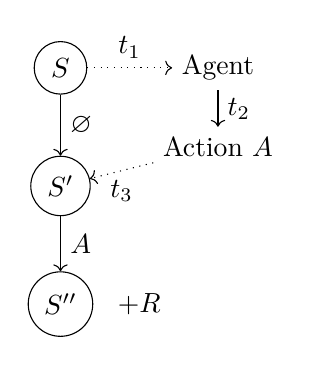
\begin{tikzpicture}
					\node[circle, draw] (state) {$S$};
					\node[circle, draw] (state') at ($(state) + (0, -1.5)$) {$S'$};
					\node[circle, draw] (state'') at ($(state') + (0, -1.5)$) {$S''$};
					
					\node (agent) at ($(2, 0) + (state)$) {Agent};
					\node[below of=agent] (action) {Action $A$};
					
					\node[right of=state''] {$+ R$};
					
					\draw[->] (state) -- (state') node[midway, right] {$\varnothing$};
					\draw[->] (state') -- (state'') node[midway, right] {$A$};
					
					\draw[dotted, ->, bend left = 30] (state) -- (agent) node[midway, above] {$t_1$};
					\draw[->] (agent) -- (action) node[midway, right] {$t_2$};
					\draw[dotted, ->] (action) -- (state') node[midway, below] {$t_3$};
					\end{tikzpicture}}};
			\end{tikzpicture}
			}
			\caption{Asynchronous RL delays and state slippage (policy updates omitted).}
		\end{figure}
	\end{column}
	\begin{column}{0.4\linewidth}
		\begin{itemize}
			\item Programmable network hardware: arbitrary in-network compute.
			\item In data-driven, want to \alert{minimise time to act}.
			\item RL assumes that action \& policy update are zero-cost.
			\begin{itemize}
				\item Not so in real deployments!
				\item State drift, etc.
			\end{itemize}
		\end{itemize}
	\end{column}
\end{columns}
\end{frame}

\begin{frame}{DDoS Prevention: VNF + SDN  architecture}
	\begin{columns}
%		\begin{column}{0.3\linewidth}
%			\begin{itemize}
%				\item Monitor flow statistics at ingress/egress points.
%				\item Use load measurements from flow paths as global state.
%				\item OUTPUT: throttle individual flows.
%			\end{itemize}
%		\end{column}
		\begin{column}{1.0\linewidth}
			\begin{figure}
				\centering
				\resizebox{0.7\linewidth}{!}{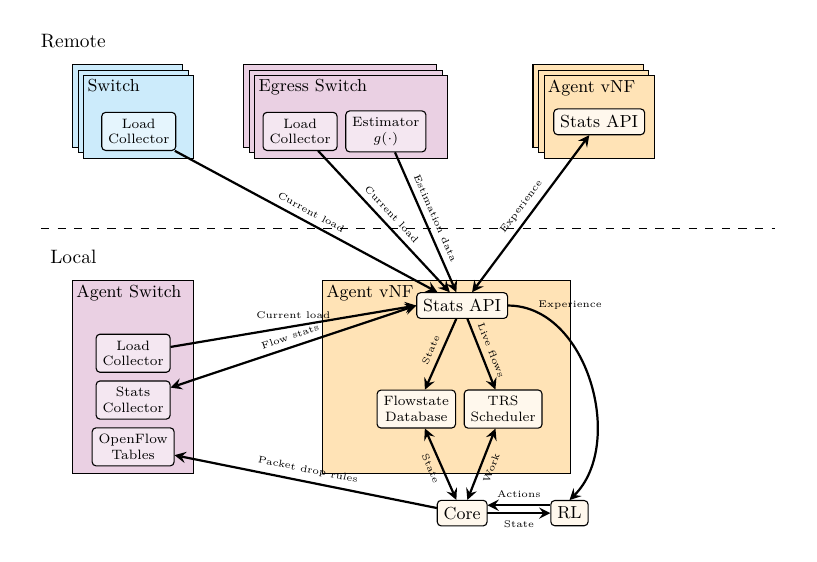
\begin{tikzpicture}[scale=1, every node/.style={scale=0.7}]
					\node(remote){Remote};
					
					%%%
					
					\node[below=0.05 of remote](swpos){};
					\node[fill=white!80!uofgcobalt, draw=black, minimum height=1.5cm, minimum width=2cm, below right= 0.1 of swpos.north west](sw1){};
					\node[fill=white!80!uofgcobalt, draw=black, minimum height=1.5cm, minimum width=2cm, below right= 0.1 of sw1.north west](sw2){};
					\node[fill=white!80!uofgcobalt, draw=black, minimum height=1.5cm, minimum width=2cm, below right= 0.1 of sw2.north west](switch){};
					\node[below right, inner sep=2pt] at (switch.north west) {\small Switch};
					\node[fill=white!90!uofgcobalt, draw, rectangle, rounded corners=0.05cm, above=0.1] (oswlc) at (switch.south) {\begin{varwidth}{1.5 cm}\scriptsize \centering Load\\Collector\end{varwidth}};
					
					%
					
					\node[right=2 of swpos](epos){};
					\node[fill=white!80!uofgthistle, draw=black, minimum height=1.5cm, minimum width=3.5cm, below right= 0.1 of epos.north west](e1){};
					\node[fill=white!80!uofgthistle, draw=black, minimum height=1.5cm, minimum width=3.5cm, below right= 0.1 of e1.north west](e2){};
					\node[fill=white!80!uofgthistle, draw=black, minimum height=1.5cm, minimum width=3.5cm, below right= 0.1 of e2.north west](egress){};
					\node[below right, inner sep=2pt] at (egress.north west) {\small Egress Switch};
					\node[fill=white!90!uofgthistle, draw, rectangle, rounded corners=0.05cm, above=0.1] (eglc) at ($(egress.south) + (-0.65,0)$) {\begin{varwidth}{1.5 cm}\scriptsize \centering Load\\Collector\end{varwidth}};
					\node[fill=white!90!uofgthistle, draw, rectangle, rounded corners=0.05cm, right=0.1] (egest) at (eglc.east) {\begin{varwidth}{1.5 cm}\scriptsize \centering Estimator\\$g(\cdot)$\end{varwidth}};
					
					%
					
					\node[right=3.5 of epos](apos){};
					\node[fill=white!60!uofgpumpkin, draw=black, minimum height=1.5cm, minimum width=2cm, below right= 0.1 of apos.north west](a1){};
					\node[fill=white!60!uofgpumpkin, draw=black, minimum height=1.5cm, minimum width=2cm, below right= 0.1 of a1.north west](a2){};
					\node[fill=white!60!uofgpumpkin, draw=black, minimum height=1.5cm, minimum width=2cm, below right= 0.1 of a2.north west](otheragent){};
					\node[below right, inner sep=2pt] at (otheragent.north west) {\small Agent vNF};
					\node[fill=white!90!uofgpumpkin, draw, rectangle, rounded corners=0.05cm, above=0.3] (oasa) at (otheragent.south) {\begin{varwidth}{1.5 cm}\small \centering Stats API\end{varwidth}};
					
					%
					
					\node[below=2.3 of remote.west](linestart){};
					\path let \p1 = (linestart) in node (lineend) at (9,\y1){};
					\draw [dashed] (linestart) -- (lineend);
					
					%%%
					
					\node[below=2.4 of remote](local){Local};
					
					%%%
					
					\node[below=0.05 of local](aswpos){};
					\node[fill=white!80!uofgthistle, draw=black, minimum height=3.5cm, minimum width=2.2cm, below right= 0.1 of aswpos.north west](aswitch){};
					\node[below right, inner sep=2pt] at (aswitch.north west) {\small Agent Switch};
					\node[fill=white!90!uofgthistle, draw, rectangle, rounded corners=0.05cm, above=0.1] (aswoft) at (aswitch.south) {\begin{varwidth}{1.5 cm}\scriptsize \centering OpenFlow\\Tables\end{varwidth}};
					\node[fill=white!90!uofgthistle, draw, rectangle, rounded corners=0.05cm, above=0.1] (aswsc) at (aswoft.north) {\begin{varwidth}{1.5 cm}\scriptsize \centering Stats\\Collector\end{varwidth}};
					\node[fill=white!90!uofgthistle, draw, rectangle, rounded corners=0.05cm, above=0.1] (aswlc) at (aswsc.north) {\begin{varwidth}{1.5 cm}\scriptsize \centering Load\\Collector\end{varwidth}};
					
					%
					
					\node[right=3 of aswpos](avfpos){};
					\node[fill=white!60!uofgpumpkin, draw=black, minimum height=3.5cm, minimum width=4.5cm, below right= 0.1 of avfpos.north west](avf){};
					\node[below right, inner sep=2pt] at (avf.north west) {\small Agent vNF};
					\node[fill=white!90!uofgpumpkin, draw, rectangle, rounded corners=0.05cm, below=0.15] (avfsa) at ($(avf.north) + (0.2,0)$) {\begin{varwidth}{1.5 cm}\small \centering Stats API\end{varwidth}};
					\node[fill=white!90!uofgpumpkin, draw, rectangle, rounded corners=0.05cm, below=0.9] (avfdb) at (avfsa.south west) {\begin{varwidth}{1.5 cm}\scriptsize \centering Flowstate\\Database\end{varwidth}};
					\node[fill=white!90!uofgpumpkin, draw, rectangle, rounded corners=0.05cm, right=0.1] (avfsched) at (avfdb.east) {\begin{varwidth}{1.5 cm}\scriptsize \centering TRS\\Scheduler\end{varwidth}};
					\node[fill=white!90!uofgpumpkin, draw, rectangle, rounded corners=0.05cm, below=2.3] (avfcore) at (avfsa.south) {\begin{varwidth}{1.5 cm}\small \centering Core\end{varwidth}};
					\node[fill=white!90!uofgpumpkin, draw, rectangle, rounded corners=0.05cm, right=0.8] (avfrl) at (avfcore.east) {\begin{varwidth}{1.5 cm}\small \centering RL\end{varwidth}};
					
					%%%
					
					\tikzset{>=stealth}
					
					\draw[thick, ->] (aswlc) -- (avfsa.west) node[midway,above] {\tiny Current load};
					\draw[thick, <->] (aswsc) -- (avfsa.west) node[midway,sloped, above] {\tiny Flow stats};
					
					\draw[thick, ->] (oswlc) -- (avfsa) node[midway,above, sloped] {\tiny Current load};
					
					\draw[thick, ->] (eglc) -- (avfsa) node[midway,above, sloped] {\tiny Current load};
					\draw[thick, ->] (egest) -- (avfsa) node[midway,above, sloped] {\tiny Estimation data};
					
					\draw[thick, <->] (oasa) -- (avfsa) node[midway,above, sloped] {\tiny Experience};
					
					\draw[thick, ->] (avfsa) -- (avfdb) node[midway,above, sloped] {\tiny State};
					\draw[thick, ->] (avfsa) -- (avfsched) node[midway,above, sloped] {\tiny Live flows};
					
					\draw[thick, ->] (avfcore) -- (aswoft) node[midway,above, sloped] {\tiny Packet drop rules};
					\draw[thick, <->] (avfcore) -- (avfdb) node[midway,below, sloped] {\tiny State};
					\draw[thick, <->] (avfcore) -- (avfsched) node[midway,below, sloped] {\tiny Work};
					\draw[thick, <-] ($(avfcore.east) + (0,0.1)$) -- ($(avfrl.west) + (0,0.1)$) node[midway,above, sloped] {\tiny Actions};
					\draw[thick, ->] (avfcore) -- (avfrl) node[midway,below, sloped] {\tiny State};
					
					\draw[thick, ->] (avfsa.east) to [out=0, in=45] (avfrl.north);
					\node[right=0.3] at (avfsa.east) {\tiny Experience};
					\end{tikzpicture}}
				\caption{
					System architecture for RL-driven DDoS defence.
					\label{fig:sys-arch}
				}
				\vspace{-1em}
			\end{figure}
		\end{column}
	\end{columns}
\end{frame}

\begin{frame}{Programmable data-planes: An Architecture for RL}
\begin{columns}
	\begin{column}{0.6\linewidth}
		\begin{figure}
			\resizebox{1.2\linewidth}{!}{\begin{tikzpicture}
				\node[fill=white!80!uofgcobalt, draw=black, minimum height=1cm, minimum width=2.9cm, below right= 0.1 of sw2.north west](p4-master){};
				\node[below right, inner sep=2pt] at (p4-master.north west) {\small P4 Master Island};
				\node[fill=white!90!uofgcobalt, draw, rectangle, rounded corners=0.05cm, above=0.1] (p4-rules) at (p4-master.south) {\begin{varwidth}{2.5 cm}\scriptsize \centering Flow Control Rules\end{varwidth}};
				
				\node[fill=white!80!uofgcobalt, draw=black, minimum height=2cm, minimum width=2cm, below = 0.1 of p4-master](sw1){};
				\node[fill=white!80!uofgcobalt, draw=black, minimum height=2cm, minimum width=2cm, below right= 0.1 of sw1.north west](sw2){};
				\node[fill=white!80!uofgcobalt, draw=black, minimum height=2cm, minimum width=2cm, below right= 0.1 of sw2.north west](switch){};
				\node[below right, inner sep=2pt] at (switch.north west) {\small P4 Island};
				\node[fill=white!90!uofgcobalt, draw, rectangle, rounded corners=0.05cm, above=0.1] (oswlc) at (switch.south) {\begin{varwidth}{1.5 cm}\scriptsize \centering Control Packet Match\end{varwidth}};
				
				\node[fill=white!80!uofgcobalt, draw=black, minimum height=2cm, minimum width=2.9cm, below= 0.1 of switch](others){};
				\node[below right, inner sep=2pt] at (others.north west) {\small Other Islands};
				\node[fill=white!90!uofgcobalt, draw, rectangle, rounded corners=0.05cm, above=0.1] (others-etc) at (others.south) {\begin{varwidth}{2.5 cm}\scriptsize \centering \textellipsis \end{varwidth}};
				\node[fill=white!90!uofgcobalt, draw, rectangle, rounded corners=0.05cm, above=0.1] (others-int) at (others-etc.north) {\begin{varwidth}{2.5 cm}\scriptsize \centering In-band Network Telemetry\end{varwidth}};
				
				\node[fill=white!80!uofgsunshine, draw=black, minimum height=5cm, minimum width=5cm](rli) at ($(p4-master.east) + (3, -2)$){};
				\node[below right, inner sep=2pt] at (rli.north west) (rli-text) {\small RL Island};
				
				\node[draw=black, dotted, minimum height=1cm, minimum width=2cm](wq-out) at ($(rli-text.south) + (0.5,-0.5)$){};
				\node[below right, inner sep=2pt] at (wq-out.north west) {\small CLS};
				\node[fill=white!90!uofgsunshine, draw, rectangle, rounded corners=0.05cm, above=0.1] (wq-in) at (wq-out.south) {\begin{varwidth}{2.5 cm}\scriptsize \centering Work Queue\end{varwidth}};
				
				\node[fill=white!90!uofgsunshine, draw, rectangle, rounded corners=0.05cm, above=0.1] (loop) at ($(wq-out.east) + (1.5,-0.5)$) {\begin{varwidth}{2.5 cm}\scriptsize \centering Control ME\end{varwidth}};
				
				\node[draw=black, dotted, minimum height=0.5cm, minimum width=2cm](policy-cls-out) at ($(loop.south) + (0,-1.5)$){};
				\node[below right, inner sep=2pt] at (policy-cls-out.north west) {\small CLS};
				\node[above right, inner sep=2pt] at (policy-cls-out.north west) {\small Policy};
				\node[draw=black, dotted, minimum height=0.5cm, minimum width=2cm](policy-ctm-out) at ($(policy-cls-out.south) + (0,-0.25)$){};
				\node[below right, inner sep=2pt] at (policy-ctm-out.north west) {\small CTM};
				\node[draw=black, dotted, minimum height=0.5cm, minimum width=2cm](policy-emem-out) at ($(policy-ctm-out.south) + (0,-0.25)$){};
				\node[below right, inner sep=2pt] at (policy-emem-out.north west) {\small EMEM};
				
				\node[fill=white!90!uofgsunshine, draw, rectangle, above=0.1, below left= 0.05] (t1) at (policy-cls-out.north east) {\begin{varwidth}{2.5 cm}\scriptsize \centering T1\end{varwidth}};
				\node[fill=white!90!uofgsunshine, draw, rectangle, above=0.1, below left= 0.05] (t2) at (policy-ctm-out.north east) {\begin{varwidth}{2.5 cm}\scriptsize \centering T2\end{varwidth}};
				\node[fill=white!90!uofgsunshine, draw, rectangle, above=0.1, below left= 0.05] (t3) at (policy-emem-out.north east) {\begin{varwidth}{2.5 cm}\scriptsize \centering T3\end{varwidth}};
				
				\node[fill=white!90!uofgsunshine, draw, rectangle, rounded corners=0.05cm, above=0.1] (po-me-1) at ($(wq-out.south) + (0,-1.0)$) {\begin{varwidth}{2.5 cm}\scriptsize \centering Policy ME\end{varwidth}};
				
				\node[fill=white!90!uofgsunshine, draw, rectangle, rounded corners=0.05cm, above=0.1] (po-me-2) at ($(po-me-1.south) + (0,-1.0)$) {\begin{varwidth}{2.5 cm}\scriptsize \centering Policy ME\end{varwidth}};
				
				\node[fill=white!90!uofgsunshine, draw, rectangle, rounded corners=0.05cm, above=0.1] (po-me-3) at ($(po-me-2.south) + (0,-1.0)$) {\begin{varwidth}{2.5 cm}\scriptsize \centering Policy ME\end{varwidth}};
				
				\draw[->] (p4-rules.west)  to [out=180,in=180,looseness=2]  node[pos=0.5, rotate=90, anchor=center, above] {Rules}(sw1);
				\draw[->] (p4-rules.west)  to [out=180,in=180,looseness=2] (sw2);
				\draw[->] (p4-rules.west)  to [out=180,in=180,looseness=2] (switch);
				
				\draw[->] (oswlc.east)  to node[midway, above, sloped] {\tiny Control, Requests} (wq-in.west);
				\draw[->] (others-int.east)  to node[midway, above, sloped] {\tiny State} (wq-in.west);
				\draw[<->, dotted] (wq-in.east)  to (loop.west);
				\draw[->, dotted] (loop.south) to (policy-cls-out);
				
				\draw[<->, dotted] (po-me-1.east) to (policy-cls-out.west);
				\draw[<->, dotted] (po-me-2.east) to (policy-ctm-out.west);
				\draw[<->, dotted] (po-me-3.east) to (policy-emem-out.west);
				
				\draw[->] (loop) to node[midway, above, sloped] {\tiny NN} (po-me-1);
				\draw[->] (po-me-1) to node[midway, above, sloped] {\tiny NN} (po-me-2);
				\draw[->] (po-me-2) to node[midway, above, sloped] {\tiny NN} (po-me-3);
				\draw[->] (po-me-3) to [out=-45,in=0,looseness=2] node[midway, above, sloped] {\tiny NN} (loop);
			\end{tikzpicture}}
			\caption{Architecture for generalised RL agent on Netronome hardware.}
		\end{figure}
	\end{column}
	\begin{column}{0.4\linewidth}
		\begin{itemize}
			\item Make decisions \alert{where they must be applied}.
			\item ``Bump-in-the-wire'' use of Netronome SmartNIC.
			\item P4 parsing/forwarding/filtering, offload to microcode for full programmability.
			\begin{itemize}
				\item P4 with offload common.
			\end{itemize}
				\item Solution: \alert{make use of on-device parallelism, externs to implement fast, adaptive data-driven applications}.
		\end{itemize}
	\end{column}
\end{columns}
\end{frame}

\end{document}